%%%%%%%% ICML 2021 EXAMPLE LATEX SUBMISSION FILE %%%%%%%%%%%%%%%%%

\documentclass{article}

% Recommended, but optional, packages for figures and better typesetting:
\usepackage{microtype}
\usepackage{graphicx}
\usepackage{subfigure}
\usepackage{booktabs} % for professional tables

% hyperref makes hyperlinks in the resulting PDF.
% If your build breaks (sometimes temporarily if a hyperlink spans a page)
% please comment out the following usepackage line and replace
% \usepackage{icml2021} with \usepackage[nohyperref]{icml2021} above.
\usepackage{hyperref}

% Attempt to make hyperref and algorithmic work together better:
\newcommand{\theHalgorithm}{\arabic{algorithm}}

% Use the following line for the initial blind version submitted for review:
\usepackage[accepted]{icml2021}
\usepackage{amsmath}
\usepackage{amssymb}
\usepackage{stmaryrd}

% If accepted, instead use the following line for the camera-ready submission:
%\usepackage[accepted]{icml2021}

% The \icmltitle you define below is probably too long as a header.
% Therefore, a short form for the running title is supplied here:
\icmltitlerunning{Reinforcement Learning 2023 Assignment 2}

\widowpenalty=10000
\clubpenalty=10000

\begin{document}

\twocolumn[
\icmltitle{Reinforcement Learning 2023, Master CS, Leiden University \\
   Assignment 2 on Deep Q Learning (DQN)}



% It is OKAY to include author information, even for blind
% submissions: the style file will automatically remove it for you
% unless you've provided the [accepted] option to the icml2021
% package.

% List of affiliations: The first argument should be a (short)
% identifier you will use later to specify author affiliations
% Academic affiliations should list Department, University, City, Region, Country
% Industry affiliations should list Company, City, Region, Country

% You can specify symbols, otherwise they are numbered in order.
% Ideally, you should not use this facility. Affiliations will be numbered
% in order of appearance and this is the preferred way.
\icmlsetsymbol{equal}{*}


\begin{icmlauthorlist}
\icmlauthor{Tom Stein (s3780120)}{lu}
\icmlauthor{Andrija Kuzmanov (s3766780)}{lu}
\icmlauthor{Tommaso Ancilli (s3674657)}{lu}
\end{icmlauthorlist}
   
\icmlaffiliation{lu}{Faculty of Science, Leiden University, Leiden, The Netherlands}

\icmlcorrespondingauthor{Tom Stein}{tom.stein@tu-dortmund.de}
\icmlcorrespondingauthor{Andrija Kuzmanov}{andrija.kuzmanov@gmail.com}
\icmlcorrespondingauthor{Tommaso Ancilli}{tommaso.ancilli@student.unisi.it}

% You may provide any keywords that you
% find helpful for describing your paper; these are used to populate
% the "keywords" metadata in the PDF but will not be shown in the document
\icmlkeywords{Reinforcement Learning, Machine Learning}

\vskip 0.3in
]

% this must go after the closing bracket ] following \twocolumn[ ...

% This command actually creates the footnote in the first column
% listing the affiliations and the copyright notice.
% The command takes one argument, which is text to display at the start of the footnote.
% The \icmlEqualContribution command is standard text for equal contribution.
% Remove it (just {}) if you do not need this facility.

%\printAffiliationsAndNotice{}  % leave blank if no need to mention equal contribution
\printAffiliationsAndNotice{} % otherwise use the standard text.

\begin{abstract}
This assignment report focuses on Deep Q Learning (DQN)
with an application to the CartPole environment. 
The basic concept of DQN is introduced along with the experience replay 
and target network improvements.
The effect of individual hyperparameters is studied empirically 
and through a hyperparameter scan.
A high degree of instability in the training process was observed, 
which is, to some extent, mitigated by specific adjustments of the parameters.
\end{abstract}

\section{Introduction}
\label{sec:introduction}
In this assignment, an agent has to learn how to balance a pole in the vertical position.
The environment presented is a well known and well-defined physical problem, being a reverse pendulum attached to a carriage through a joint.
The goal of this learning task is to keep the pole in place while moving the cart left or right.
The possible action space is made up by a set of only two possible movements $\{0,1\}$, where $0$: the cart is pushed to the left; $1$: the cart is pushed to the right.
The state space is composed of four values: position and velocity of the cart, angle and angular velocity of the pendulum.
The agent receives a reward of $+1$ for every action performed that results in keeping the pole in an upright state ($\pm 12^\circ$).
The environment is reset to the initial condition every time that the value of the angle between the pole and the vertical line is bigger than $12^\circ$ or when the cart leaves the range horizontal range $(-2.4;2.4)$.
The maximum reward in the environment is limited to 500 because there is no natural end to the balancing problem, and obtaining a reward of 500 demonstrates the ability to balance the pole quite well.

The old paradigm, where all the q-values could be stored in a table and updated directly to determine the optimal policy, is not suitable anymore.
The reason lies in the exponential amount of memory required to store all the possible states (curse of dimensionality).
Given the impossibility of memorizing all the possible states, the agent has to learn how to generalize to unseen data.
This can be done through the application of deep learning.
It is known that an Artificial Neural Network has the property to approximate any function~\cite{Cybenko}, enabling the possibility of inferring an unseen state and having a more compact representation of the solution itself.
The resulting algorithm, generated by the union of Deep learning and Q-learning, is called Deep Q-Network algorithm (DQN).
In this report, the neural network has to approximate the Q-values using a parameterized function.
This approach is also called value-based.

\begin{equation}
    Q_{\theta} :  s \rightarrow q
    \label{eq:value-based-approach}
\end{equation}
where, $s \in S$ where $S$ represents the set of all the possible states and $q$ is the Q-values of the admissible actions.


The remaining chapters are structured as follows.
In \autoref{sec:background}, the underlying concepts regarding the separate approaches will be shown.
Following that, the results from an actual implementation of these concepts are shown in \autoref{sec:results}. 
That section primarily investigates the influence of individual hyperparameters on the performance of the agent.
Afterwards, a comprehensive hyperparameter scan is conducted to study the relationship between hyperparameters in \autoref{sec:bonus}.
Finally, in \autoref{sec:discussion} the results are summarized and insights into what could have been improved are given.


\section{Background}
\label{sec:background}
This section will examine methods used to solve the cart pole balancing problem.
Ideally, the problem would be solved with the Q-learning method, since it is easy to implement and interpret.
However, due to continuous state space it is not possible to store a $Q(s,a)$ value for every state-action pair.
Because of that, the deep learning methods will be used to estimate the $Q(s,a)$ value for any given state-action pair.
Firstly, the DQN or Deep Q-learning method will be examined.
Secondly, the DQN method will be improved with experience replay and a target network.

\subsection{DQN}
\label{subsec:dqn}
Deep Q Learning (DQN) is one of the most known deep reinforcement learning algorithms.
It is based on the tabular Q-learning method, but instead of obtaining the $Q$ value from a table,
a neural network is trained (the parameters are adjusted) to predict the values given a certain state.
A neural network is a machine learning structure that contains a large amount of parameters that can be tuned
to represent a certain function.
The DQN agent learns by taking steps in the environment and updating the $Q$ value estimates by using the obtained reward.
The update process is called bootstrapping, as it refines the old estimates using new updates~\cite{DBLP:books/sp/Plaat22}.
In order to update the current $Q(s,a)$ value, first a step is taken, reward is obtained, and the (expected)
target value $GT$ of $Q(s,a)$ is computed with the following equation:

\begin{align}
   \label{eq:calculating-target}
    GT = r + \gamma \cdot \max_{a^\prime} Q_{\theta}(s^\prime, a^\prime)
\end{align}

From \autoref{eq:calculating-target} it can be seen that the target is based on the received reward and the discounted
value of the next state.
The letter $\gamma$ represents the discount factor and the letter $\theta$ represents the parameters of the neural network $Q$.
The target and our current $Q(s,a)$ estimate can then be used to compute the loss using a pre-defined loss function.
A loss function can be any mathematical function that measures the difference between the predicted output and the
actual output.
One of the most common examples when it comes to regression problems is the mean squared error function displayed
in \autoref{eq:mse}, 
where $x$ and $y$ denote the predicted and the actual values, while $n$ denotes the number of values.

\begin{align}
   \label{eq:mse}
   \alpha(x, y) = \frac{1}{n} \cdot \sum_{i = 0}^{n} [(x_i - y_i)^2]
\end{align}

Using the computed loss, the parameters $\theta$ can be optimized in order to minimize the loss.
One of the most common algorithms for optimization is called stochastic gradient descent (SDG).
It computes the gradient of the loss function with respect to the parameters $\theta$.
The gradients are then used to push each of the parameters in the opposite direction of the gradient and with that minimize
the loss.
The amount by which each of the parameters is pushed is determined by the learning rate $\alpha$.
The smaller the $\alpha$ the smaller the step taken in the opposite direction of the gradient.
In the experiments conducted in this report, the Adam optimizer is used, which tries to improve upon the SDG optimizer
by using the first and the second moments of the gradient to adapt the learning rate for each weight
of the neural network~\cite{kingma2014adam}.

The algorithm~\ref{alg:dqn} displays how a DQN algorithm learns.
Similar to regular Q learning, there are two loops.
The first loop defines the amount of the episodes that need to be executed, and the second loop executes
the episode until termination.
While performing an episode, first an action must be picked based on the $Q$ value estimates,
that are obtained by passing the current state $s$ to the neural network.
Because of this, the estimates will be completely random in the beginning, but will improve as more moves are made and learned.
Different policies for action-selection can also be used, for example, epsilon-greedy or the Boltzmann policy
whose parameters can be tuned to incorporate a balance between exploration and exploitation.

After obtaining an action, it can then be executed inside the environment in order to obtain the next state $s^\prime$
as well as the reward $r$ for performing that action.
Afterwards, the $Q(s,a)$ value and the target estimate can be computed (using \autoref{eq:calculating-target}).
The loss is equal to the squared difference between the target $Q$ value and the $Q(s,a)$ value that was computed.

Once terminal state is reached, the gradient of the loss function with respect to the neural network's parameters is calculated.
Those gradients are then provided to the backward pass function that optimizes the parameters.


\begin{algorithm}
   \caption{DQN pseudocode}
   \begin{algorithmic}
      \REQUIRE environment, Qnet, $\alpha \in (0,1]$, $\gamma \in [0,1]$, $\epsilon \in [0,1]$, max\_epoch $\in$ $\mathbf{N}$
      \STATE $s = s_0$ \COMMENT{Initialize start state}
      \FOR{i = 0..max\_epoch}
         \STATE sum\_sq = 0
         \WHILE{$s$ not TERMINAL}
            \STATE $a$ = select\_action(Qnet(s))
            \STATE $s^\prime$, $r$ = env.step($a$)
            \STATE output = max(Qnet($s$))
            \STATE target = $r$ + $\gamma \cdot$ max(Qnet($s^\prime$))
            \STATE sum\_sq += $(target - output)^2$
            \STATE $s = s^\prime$
         \ENDWHILE
         \STATE grad = Qnet.gradient(sum\_sq)
         \STATE Qnet.backward\_pass(grad, $\alpha$)
      \ENDFOR
      \STATE \textbf{Return:} Qnet
   \end{algorithmic}
   \label{alg:dqn}
\end{algorithm}

While the algorithm seems promising, it still faces three important challenges.
Firstly, the convergence of the algorithm depends on the full coverage of the state space, which in the case of the described
problem is just not feasible.
Secondly, there is a strong correlation between subsequent training samples that can lead to poor generalization and overfitting.
Thirdly, a bootstrapped target is used to calculate the loss of each prediction.
The weights of the network that predicts the target change after every optimization step, which can lead to unstable learning~\cite{DBLP:books/sp/Plaat22}.

The problems posed in the previous paragraph can not be fully solved, but it is possible to minimize their impact.
Firstly, the problem of low coverage can be improved by setting a high probability of taking an exploratory step.
The higher the probability, the higher amount of state space the algorithm will explore.
Secondly, the high correlation problem can be improved by implementing experience replay, which is described in \autoref{subsec:experience-replay}.
Thirdly, a secondary neural network that is updated less frequently can be implemented and used only for target predictions.
This approach is called target network and is explained in \autoref{subsec:target-network}
Finally, the learning can be stabilized by setting a very low learning rate $\alpha$ that will minimize the change between
subsequent target predictions.

\subsection{Experience Replay}
\label{subsec:experience-replay}
The plain DQN algorithm suffers from high correlation between subsequent states, e.g., if the agent performs good and the environment does not change much.
This means that the agent frequently visits similar states and makes similar actions,
and consequently trains the neural network on very similar samples.
What is more, because of bootstrapping and function approximation, the algorithm can forget some useful behaviour that it learned in the past.
This can lead to overfitting, instability in the training process and consequently poor generalization.
Moreover, it may also fail to cover a significant amount of state space and get stuck
in the local optima because of this.
To break the correlation, one can make use of a concept called experience replay (ER).
The ER adds a replay buffer, a buffer that stores experiences in the form of $T=(state, action, reward, next\_state)$ transition tuples, that can be used to break the correlation.
Using this, the DQN agent no longer needs to learn from subsequent experiences, as it can obtain random samples
from the replay buffer and learn from them instead.
Breaking the correlation between subsequent samples improves coverage and generalization of the algorithm~\cite{DBLP:books/sp/Plaat22}.
Without this, DQN can become biased towards the most recent experiences and forget the previous experiences
that are still very relevant for the task.

\subsection{Target Network}
\label{subsec:target-network}
In order to improve the stability of learning and reduce the divergence caused by frequent weight updates,
a target network can be introduced~\cite{DBLP:books/sp/Plaat22}.
Target network (TN) $\hat Q$ is a new neural network that the algorithm will use to output the target values.
The newly added network is structurally a copy of the value network $Q$, but it gets updated every $n$ steps
by copying the parameters of the neural network $Q$ that is used for action selection ($\hat Q = Q$).
That way, the target predictions remain stable for a longer period of time.
To calculate the target value, the \autoref{eq:calculating-target} can still be used, however, instead of using the $Q_\theta$
neural network it needs to be replaced with $Q_{\theta - i}$ neural network where $\theta - i$ stands for the parameters
which were used $i$ steps ago.
In this case, the variable $i$ stands for the number of time steps since the target neural network $\hat Q$ was last updated.
After every $n$ steps, the $\hat Q_{\theta - i}$ is updated, making the variable $i$ equal to 0 and $\hat Q_{\theta - i}$
equal to $Q_\theta$.

\section{Results}
\label{sec:results}
This section presents the results obtained by tuning the most important hyperparameters individually. 
In \autoref{subsec:dqn-ablation-study}, the effect of experience replay and a target network are investigated.
In order to have a common baseline for comparisons, a set of hyperparameters was defined as shown in \autoref{tbl:baseline_config}. 
These values will be used throughout this section, if not mentioned otherwise explicitly.
The values were chosen based on prior experiments and experience.
To account for the inherent randomness in our experiments,
we decided to run each combination of hyperparameters five times as a compromise between statistical significance and the computational power required to perform the experiments. The same number of repetitions is done in every plot of this section if not mentioned otherwise.\\
To express the confidence in our results, the graphs are portrayed the mean value - bold line- and the standard deviation - the faded interval surrounding the mean value.   

\begin{table}[ht]
   \caption{Baseline hyperparameter values. Assume these values for any hyperparameter throughout this section if not mentioned otherwise.}
   \label{tbl:baseline_config}
   \vskip 0.15in
   \begin{center}
   \begin{small}
   \begin{sc}
   \begin{tabular}{lcccr}
   \toprule
   Parameter & Value \\
   \midrule
   Network Architecture    & $4-64-32-32-2$ \\
   Learning rate           & $0.001$ \\
   Learning rate decay     & $1.0$   \\
   Epochs                  & $1000$ \\
   Policy                  & epsilon greedy \\
   Initial epsilon         & $0.2$ \\
   Epsilon Decay           & $0.99$ \\
   Minimal epsilon         & $0.01$ \\
   Gamma                   & $0.9$ \\
   Batch size              & $2$ \\
   Buffer size             & $500000$ \\
   \bottomrule
   \end{tabular}
   \end{sc}
   \end{small}
   \end{center}
   \vskip -0.1in
\end{table}

To verify that the agent actually learned something, 
we investigated the performance of a random agent, 
i.e. an agent that performs any action uniformly random. 
The random agent achieved an average cumulative reward of 22.4 per episode (see \autoref{fig:random_agent}).
Any performance below this threshold is worse than taking random actions 
and can be considered bad.


\begin{figure}[ht!]
   \centering
   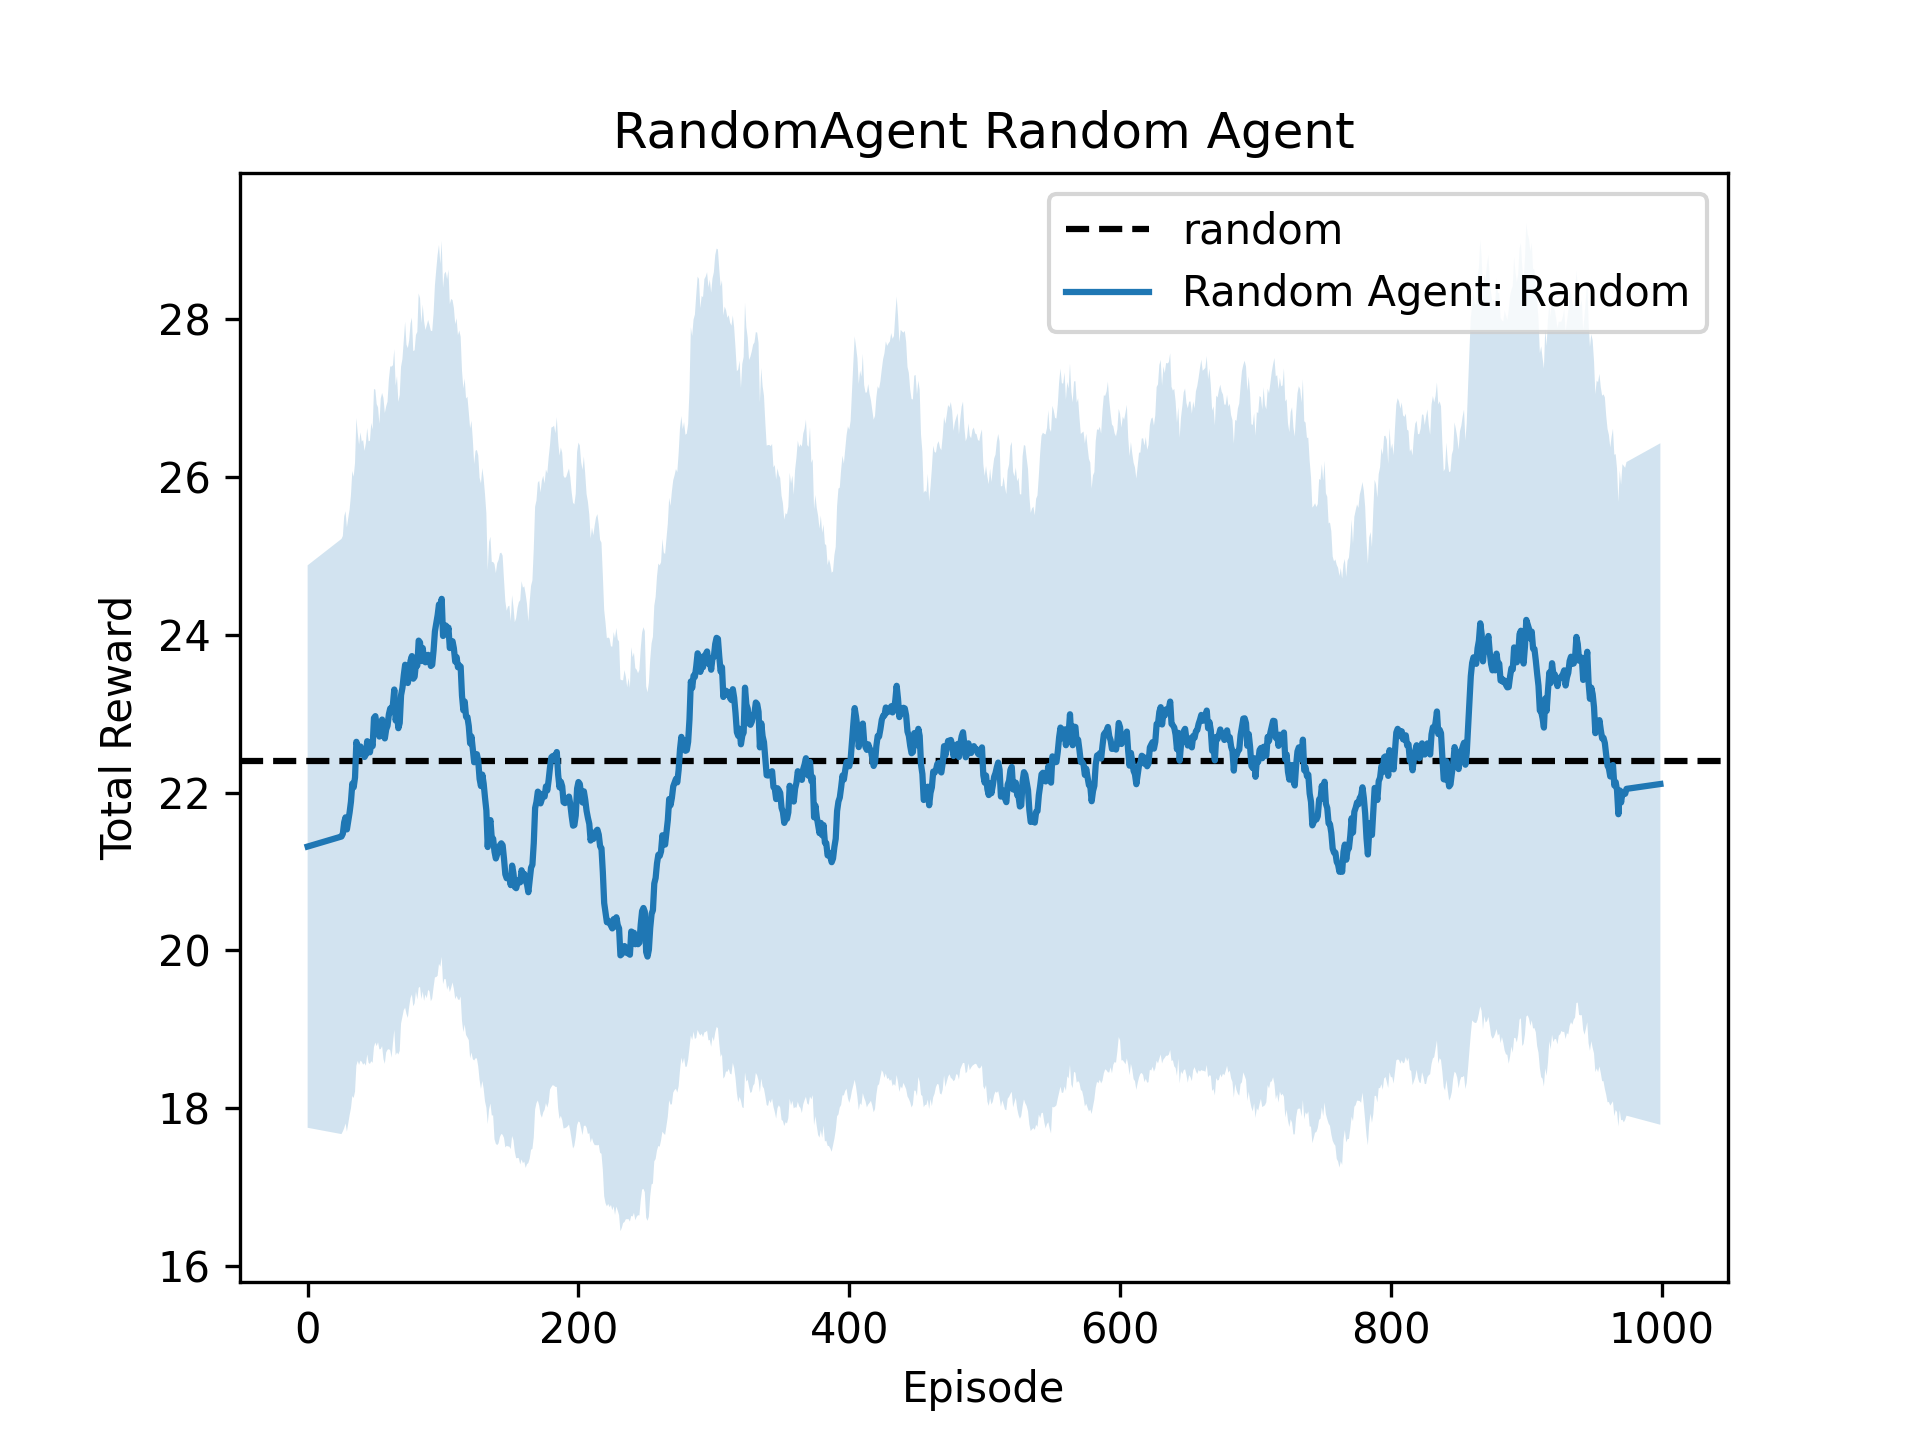
\includegraphics[width=0.3\textwidth]{assets/random_agent_cumulative_reward.png}
   \caption{The smoothed cumulative reward per episode of a random agent is shown 
      along with the standard deviation. The global average of 22.4 is indicated by the black dotted line.
   }
   \label{fig:random_agent}
\end{figure}

\subsection{DQN with ER and TN}
\label{subsec:dqn-with-er-and-tn}

% Explain methodology
%     Number of repetions was choosen as 5 as a trade-off between statistical significance and computation time
%     Choose of baseline parameters (our educated guesses from some prior runs)
%        - Epochs = 1000
%     Why parameters we varied and what ranges
%        - Buffer size in the range up to 500k (because that is the limit given by 1000 Epochs * 500 steps)

Five different learning rates have been taken into account to detect the best one \autoref{fig:comp_learning_rate}. 
Beginning our consideration with the highest value of $0.1$, it can be clearly seen how this value is not suitable at all, 
leading the agent to receive an average reward that does not even reach the performance of a random agent. 
A learning rate of $0.01$ leads the agent to learn relatively quickly in the first hundreds of episodes, 
but the progression is not sustained in the remaining parts. 
Indeed, after the cumulative reward reaches its peak around the $190^{th}$ episode, in the remaining episodes, the number of moves performed by the agent varies within a range of $75$ and $30$, exhibiting an oscillatory behavior. 
A learning rate of $10^{-4}$ leads to a performance that is comparable to the ones of $5 \cdot 10^{-4}$ and $10^{-3}$ after 1000 epochs. 
However, the learning process is considerably slower, as one would expect.
The learning rates of $5 \cdot 10^{-4}$ and $10^{-3}$ show the best performance in terms of peak reward and computation time. 
As expected, the slightly larger learning rate of $10^{-3}$ 
receives higher rewards in the first two hundred episodes. 
However, letting the episodes go on, we can clearly see how $5 \cdot 10^{-4}$ outperforms the other value.
After all, we deem $5 \cdot 10^{-4}$ to achieve the best performance out of the five learning-related that were considered.

\begin{figure}[ht!]
   \centering
   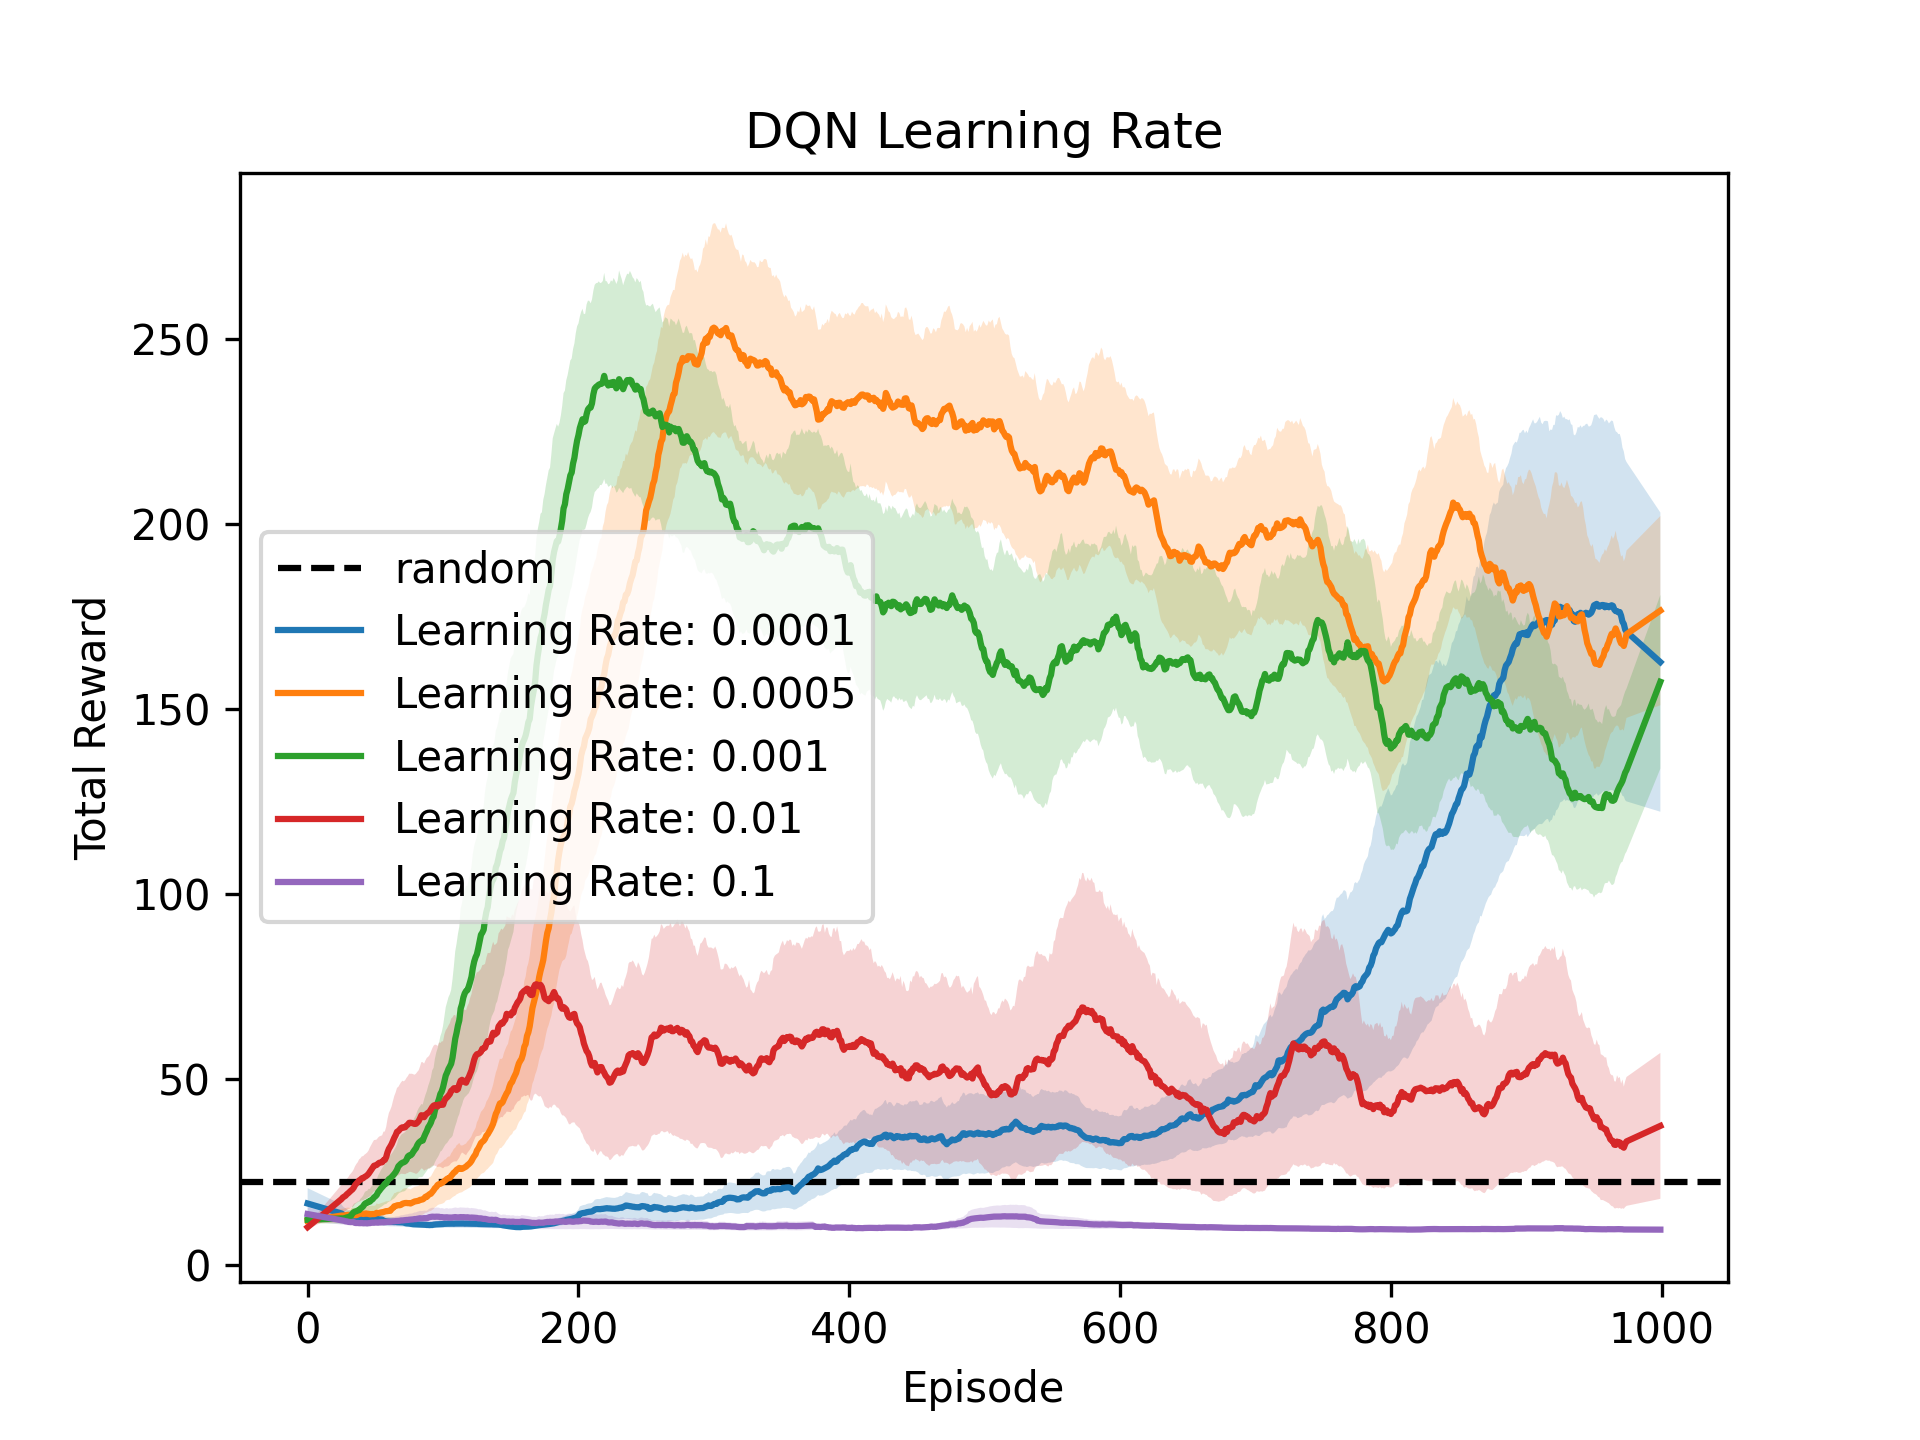
\includegraphics[width=0.3\textwidth]{assets/fig_hp/learning_rate.png}
   \caption{Comparison between five different learning rates. 
   }
   \label{fig:comp_learning_rate}
\end{figure}
 
   Concerning the architecture for the neural network, we have decided to restrict our search-guess into finding the best MLP (MultiLayer Perceptron) architecture.
   Five different architectures have been tested as the \autoref{fig:comp_nn_arch} reports. 
   In each of the different architecture the number of hidden layers and neurons is chancing. 
   After taking a closer look at the results, we can already discard the architecture $4-32-128-256-2$ since it performs poorly. 
   The other mirrored architecture, $4-256-128-32-2$, has the same performance of the smaller ones, and for this reason the Occam's razor was used as a principle to discard them.\\
   For the same principle the architecture with $4-64-32-32-2$ is preferred over $4-32-64-64-2$. 
   We have decided to adopt the architecture $4-128-128-2$ over $4-64-32-32-2$ because of its good trade-off between depth, performance and size. 
   Indeed, the computational time was almost the same, but having more parameters, we were confident that it would be able to generate a more abstract information about the data.\\
   \begin{figure}[ht!]
      \centering
      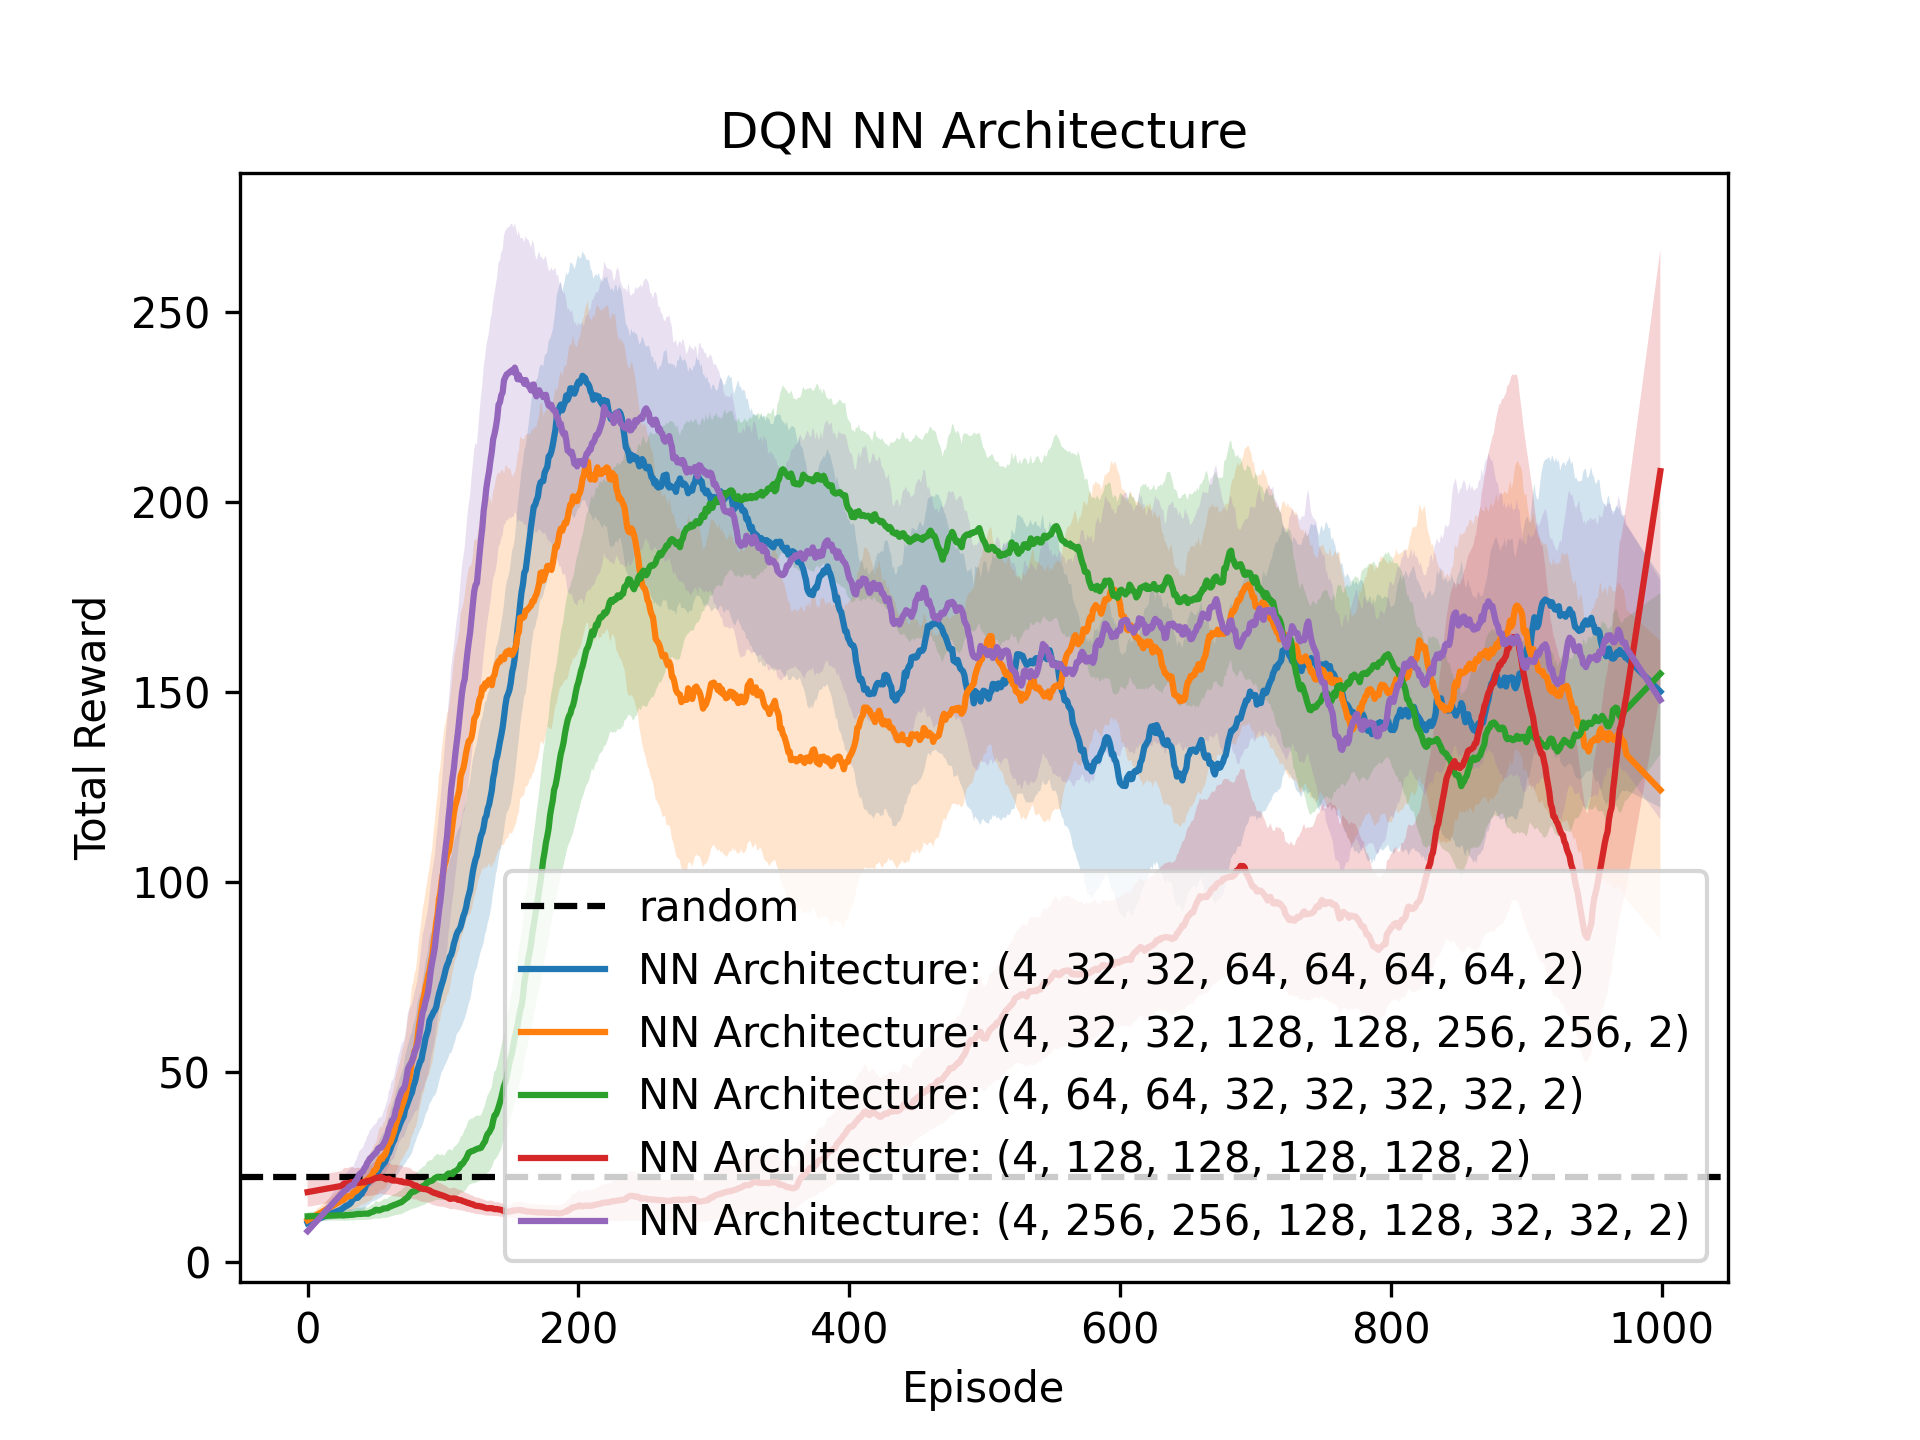
\includegraphics[width=0.3\textwidth]{assets/fig_hp/nn_architecture.png}
      \caption{Comparison between five different architectures. 
      }
      \label{fig:comp_nn_arch}
   \end{figure}

   As an action selection, these two graphs show the comparison between $\epsilon$-greedy and Boltzmann. 
   Starting with looking at the reward trend as the $\epsilon$ \autoref{fig:comp_epsilon} varies, 
   it can be seen that at the beginning having a high degree of exploration can allow the agent to perform better. 
   In fact, up to the 200th episode, the best values are when $\epsilon$ is $0.2$ or $0.5$.  
   The oscillatory and random pattern is a peculiar characteristic of all four possible combinations. 
   In fact, up to the nine-hundredth repetition they all turn out to be very similar. 
   The one that turns out to be the best is $\epsilon$ = $0.1$.\\
   A completely different discussion applies to the study of the optimal temperature parameter \autoref{fig:comp_temp}. 
   In this case, the only parameter we can use as a discriminant is the value of moves we obtain at the end of the episodes. 
   According to our metric, the best value for the hyperparameter is equal to $1$. Under this assumption, the Boltzmann function becomes the softmax function. 

   %TODO: HOW TO CREATE TWO FIGURE IN THE SAME IMAGE
   % We should only put them into the same figure if that figure spans both columns. Otherwise the images will be too small.
   \begin{figure}[ht!]
      \centering
      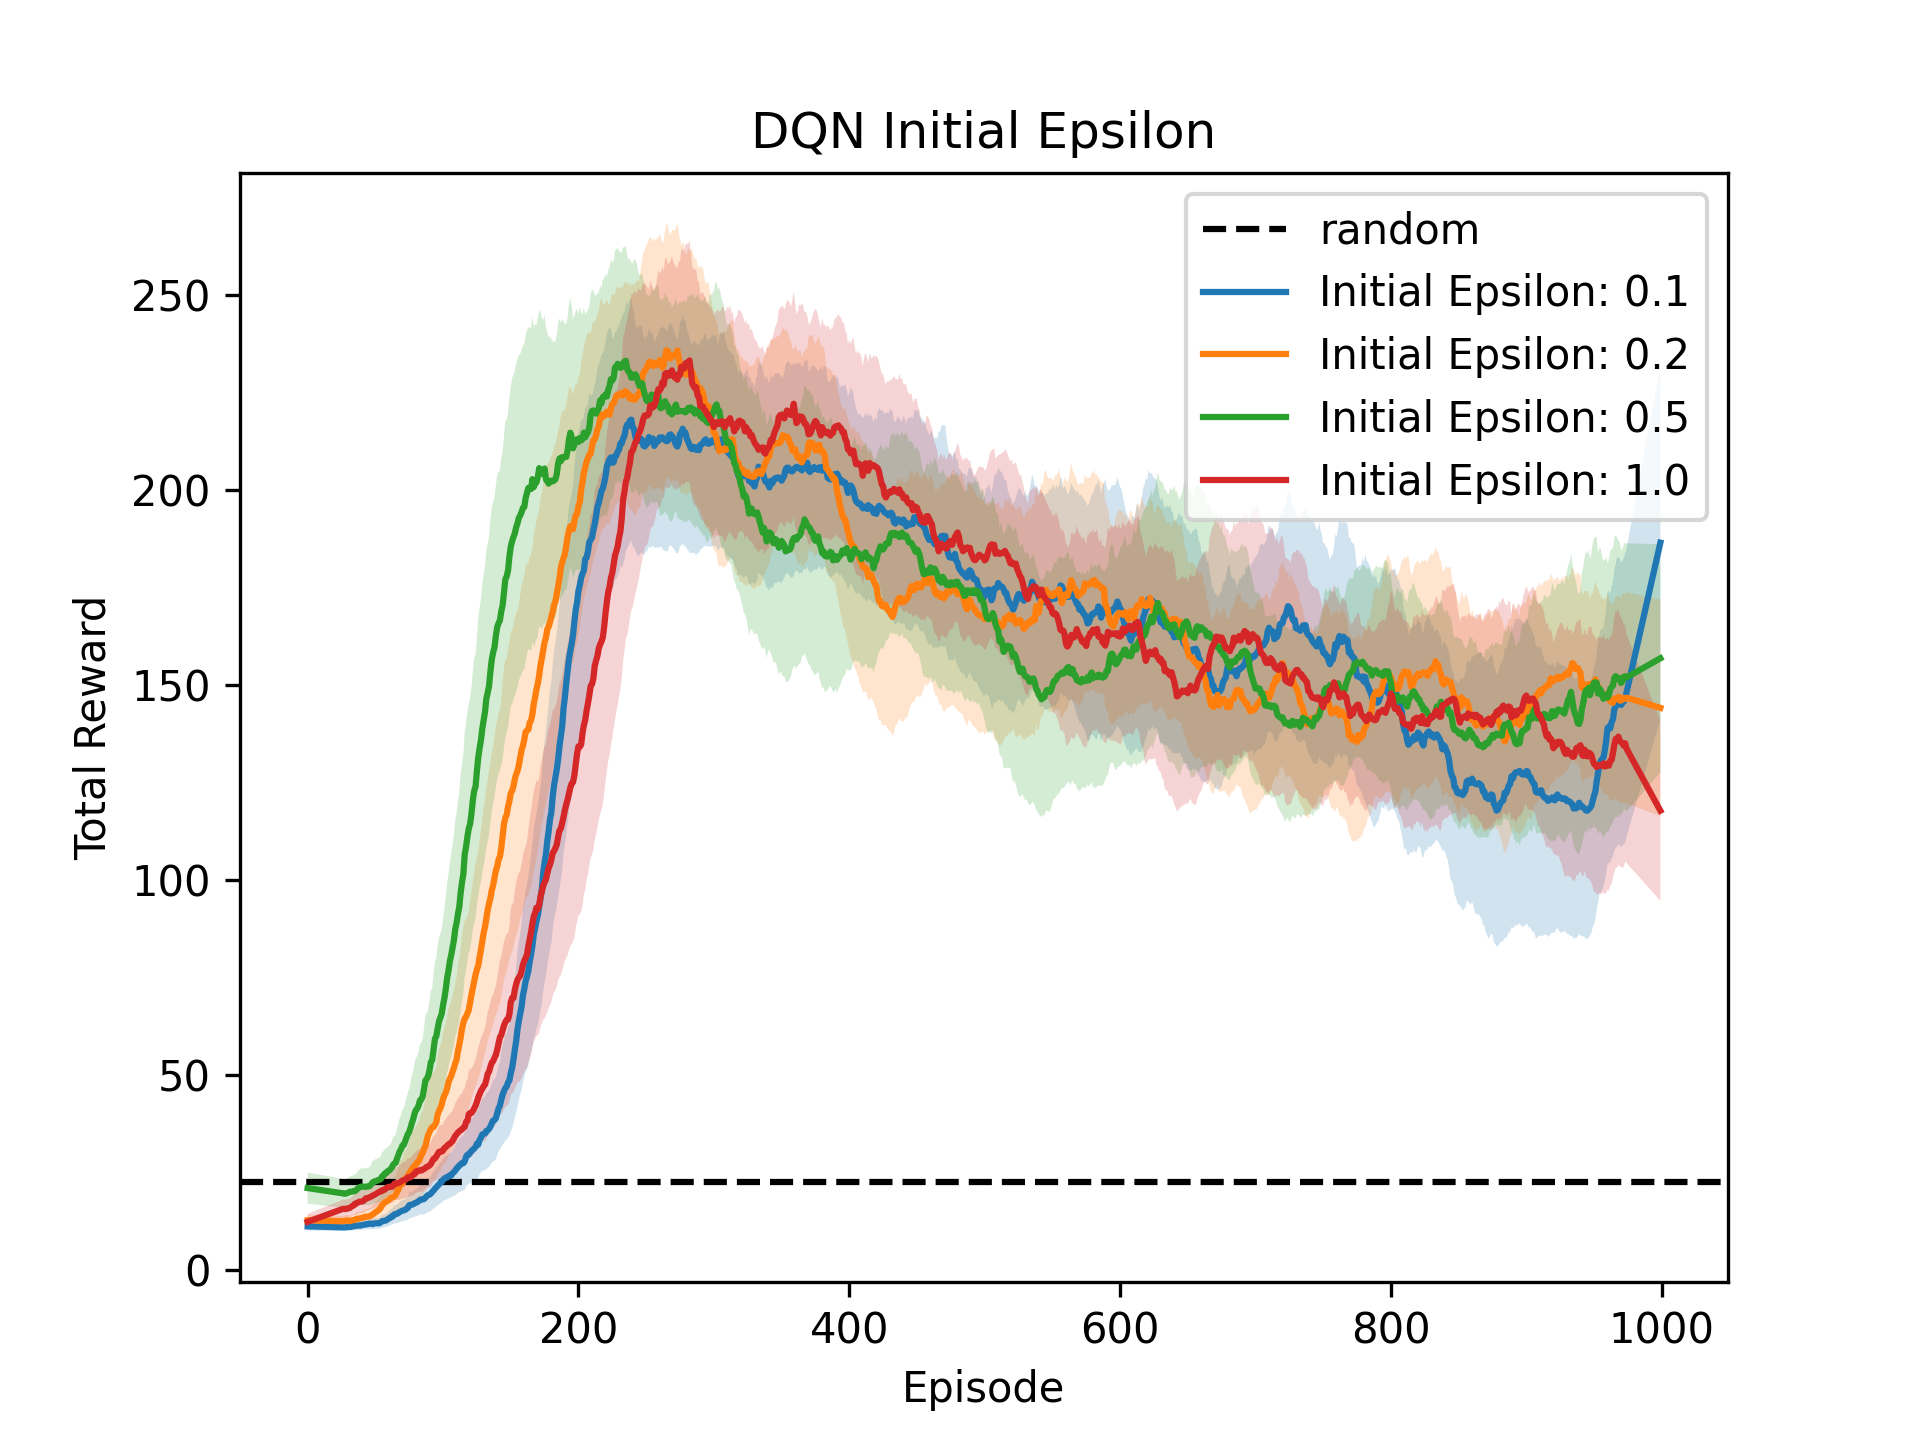
\includegraphics[width=0.3\textwidth]{assets/fig_hp/epsilon.initial.png}
      \caption{Comparison between five different architectures.
      }
      \label{fig:comp_epsilon}
   \end{figure}

   \begin{figure}[ht!]
      \centering
      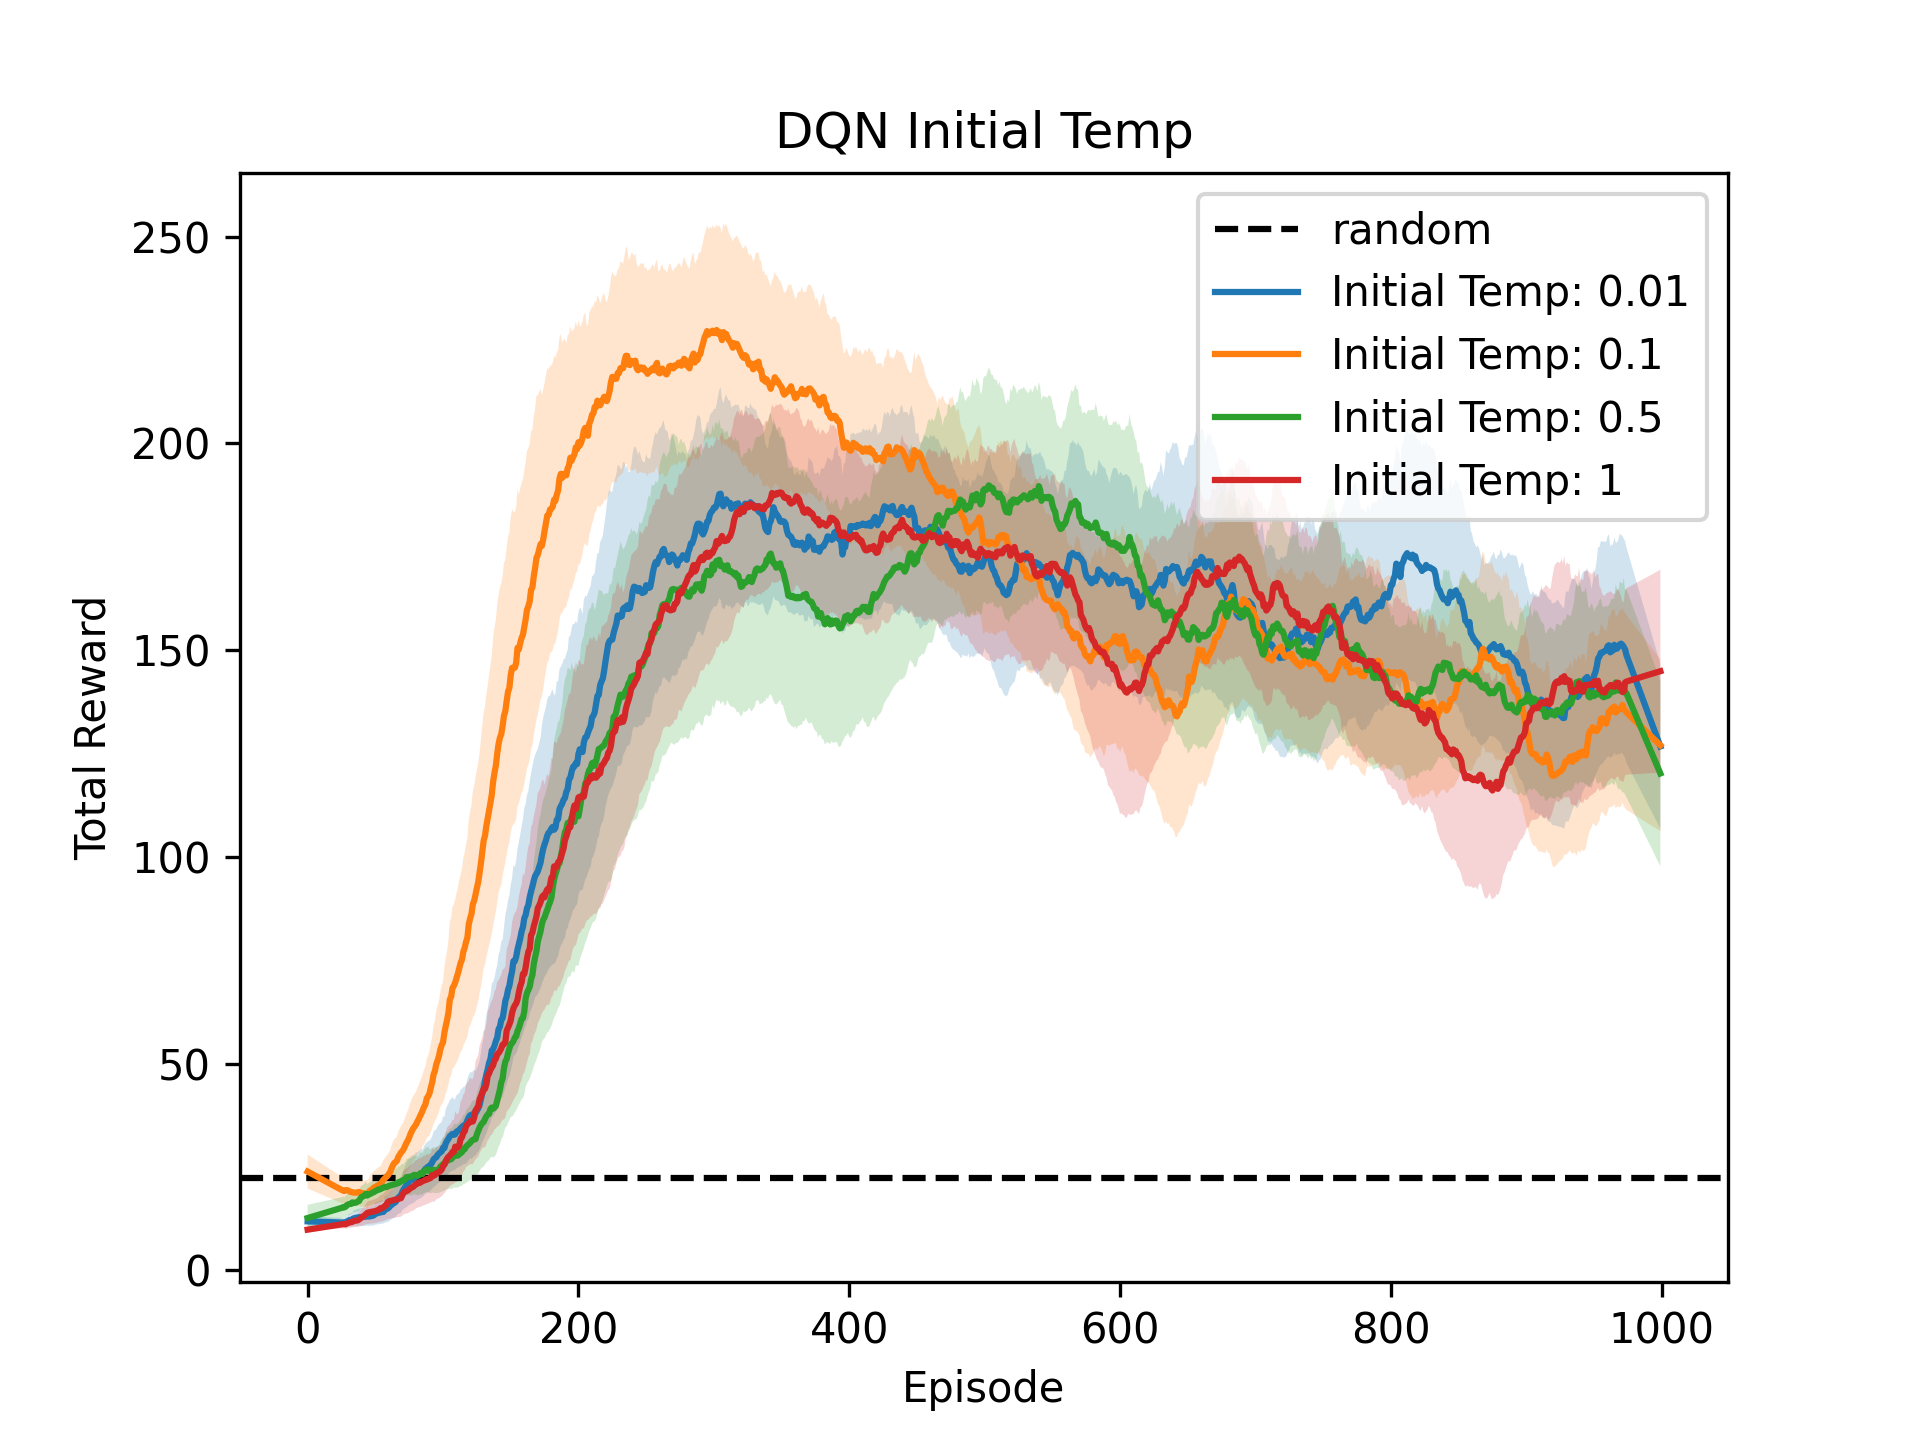
\includegraphics[width=0.3\textwidth]{assets/fig_hp/temp.initial.png}
      \caption{Comparison between five different architectures.
      }
      \label{fig:comp_temp}
   \end{figure}


% TODO: Mention catastropic forgetting

\subsection{DQN ablation study}
\label{subsec:dqn-ablation-study}
In this subscetion we ablation study is performed \autoref{fig:ablation_study}. 
After having found the best configuration for the hyperparameters, we are comparing the different solutions to improve the DQN algorithm.\\
The plain approach, where both Experience Replay and Target Network have been disabled, records the worst performances, unsurprisingly. 
Our reasoning brought us to indicate as the deadly triad, confirming the theory already expressed in \cite{DBLP:books/sp/Plaat22} and \autoref{subsec:dqn}.\\
The third approach in term of goodness of the model is the DQN algorithm which has only the target network activated. 
This solution aims to reduce the divergence, which is one of the elements of the deadly trio. \\
A possible explanation as to why the model with only the target network only slightly outperforms the basic model lies in parameter tuning. 
In our opinion, the values found were taken on the basis of the model with both the target network and the replay buffer active and were not optimal in this configuration. \\
The model that has the replay buffer active manages to achieve a decent performance. By having a buffer size of $10000$ we are able to effectively reduce the dependency between two successive states \cite{DBLP:books/sp/Plaat22}. 
It should be noted that compared to the previous models, the latter two have a very slow initial training phase and only after many epochs manage to pass the threshold.\\
Finally, the final analysis focuses on the last model. The data collected reinforce the theoretical foundations studied during the course. 
In fact, it is evident how the joint combination of the replay buffer and the target network succeeds in limiting the harmful effects of the deadly triad -  \cite{DBLP:books/sp/Plaat22} and \autoref{subsec:dqn}. 
In fact, despite a slight stochastic phase in which the total reward per epoch is lower than in the model with only the replay buffer active, the complete model visibly performs better. \\

\begin{figure}[ht!]
   \centering
   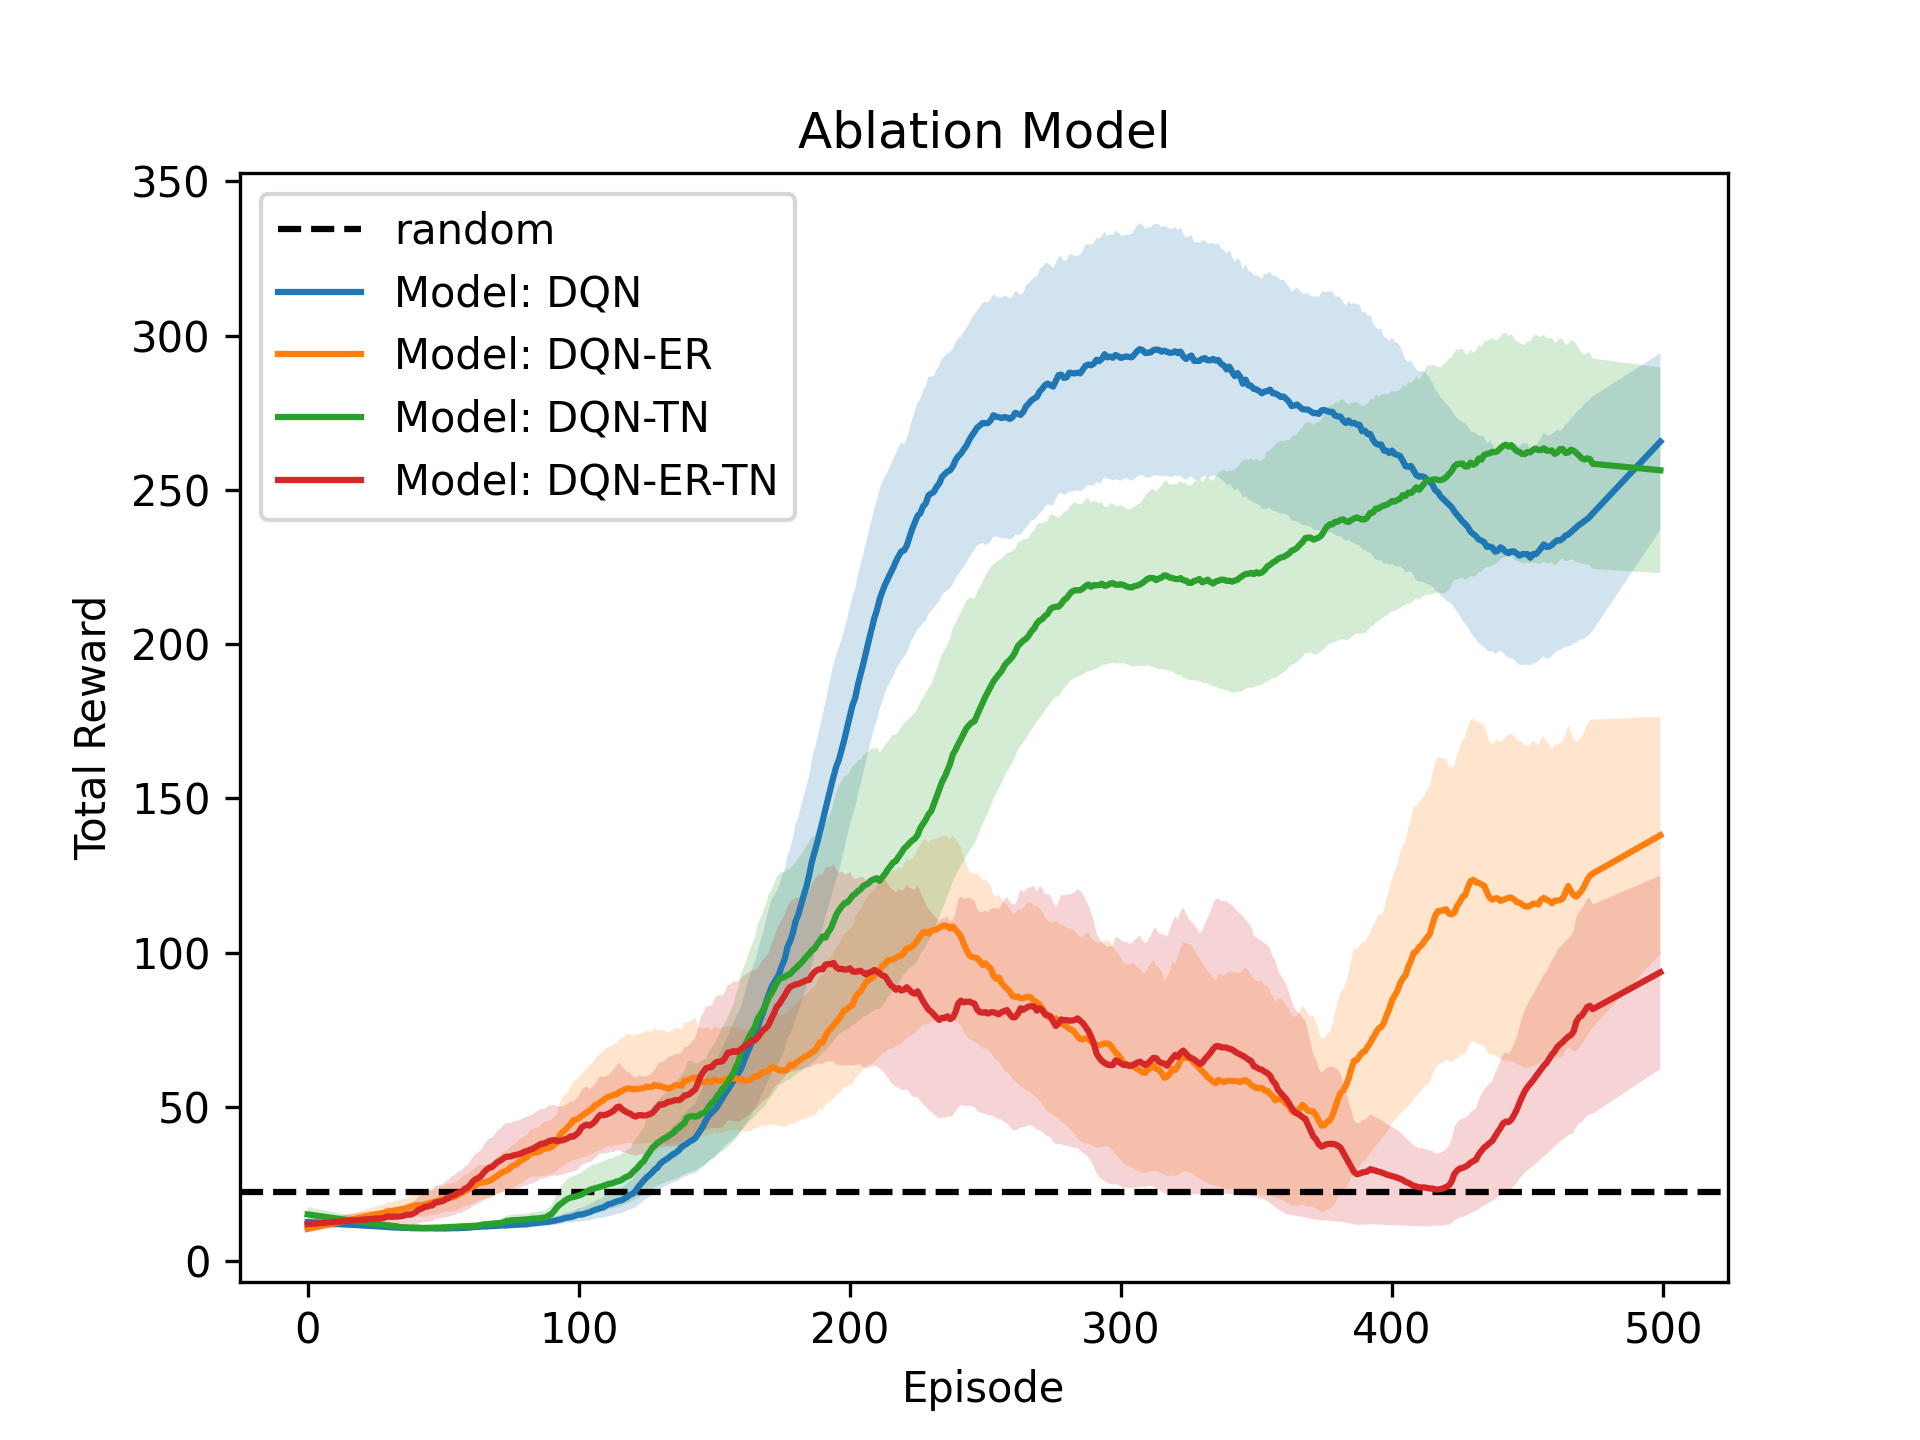
\includegraphics[width=0.3\textwidth]{assets/Ablation/ablation_study.png}
   \caption{Ablation study between four different approaches. 
   }
   \label{fig:ablation_study}
\end{figure}


\section{Hyperparameter Scan - Bonus}
\label{sec:bonus}
So far, only some individual hyperparameters were analyzed in isolation in \autoref{sec:results}.
This approach does not take into account the dependencies between the different hyperparameters 
such as learning rate and batch size~\cite{DBLP:conf/iclr/SmithKYL18}.
Additionally, some hyperparameters such as learning rate decay, experience buffer size and target network sync frequency have not been investigated at all.
For this reason, a comprehensive hyperparameter scan was performed, in which DQN models with ER and TN were trained on random combinations of the hyperparameters. 
The definition of the hyperparameter search space\footnote{\texttt{wandb\_sweep\_config.yaml}} 
intentionally does not make use of continuous value ranges like $[0.8, 1.0]$ but a preselection of discrete values to be able to group and plot the results more easily.
The hyperparameter space contains about 300 million combinations and is too large to be fully searched (i.e. grid search). 
Therefore, a random search in combination with parallel experiments were used to search this large space in a reasonable time.
To support this, the platform Weights and Biases~\cite{wandb} was used to log\footnote{\texttt{wandb\_run.py}} all experiments and to orchestrate the hyperparameter scan across multiple computers.
The results are shown in \autoref{sec:hyperparameter-scan-results},
but can also be viewed interactively online\footnote{\url{https://api.wandb.ai/links/rl-leiden/udme67qe}}. 
In total 166 parameter combinations were evaluated in 6 days compute time.


Unfortunately, only a few runs (166), with respect to the hyperparameter space size, could be collected due to time limitation.
Therefore, all the insights have to be taken with care since there is not much statistical support for them.
Furthermore, it must be ensured that policy-specific parameters such as the initial epsilon value or the initial temp value are only evaluated for runs in which the corresponding action selection policy has been applied. 
Otherwise the results are arbitrary, because the parameters are not used at all.
Additionally, it must be taken into account that the model's performance shown in the parallel axis plot 
\autoref{fig_hyperparameter_scan_parallel_axis} is solely based on the performance in the last 100 epochs (900-1000) 
and does not reflect and prior good or bad performance.

Nevertheless, we carefully analyzed the data and found the following three findings.
Firstly, the results again illustrate the instability caused by wrong parameter selection or catastrophic forgetting, 
since numerous runs only achieve poor results, much worse than a random agent. 
Secondly, the results of the hyperparameter scan, when considered in isolation, 
support most of the findings from \autoref{sec:results}. 
For example, a larger experience buffer size again shows a significant improvement in performance (see \autoref{fig:hyperparameter_scan_isolated_buffer_size})
as it was found by \cite{DBLP:conf/icml/FedusRABLRD20} too. 
Similar support can be found for the learning rate and the initial exploration factor values.
However, it was found that a gamma value of 1.0 works better than all the others, 
which is a contradictory result to the previously found behavior with a similar gamma value of 0.99 (see \autoref{fig:hyperparameter_scan_isolated_gamma}).
This could be explained by the interference with other hyperparameters
Thirdly, no significant dependency between any two parameters could be found.
Hypotheses such as a correlation between learning rate and batch size could not be identified. 

\begin{figure}[ht!]
   \centering
   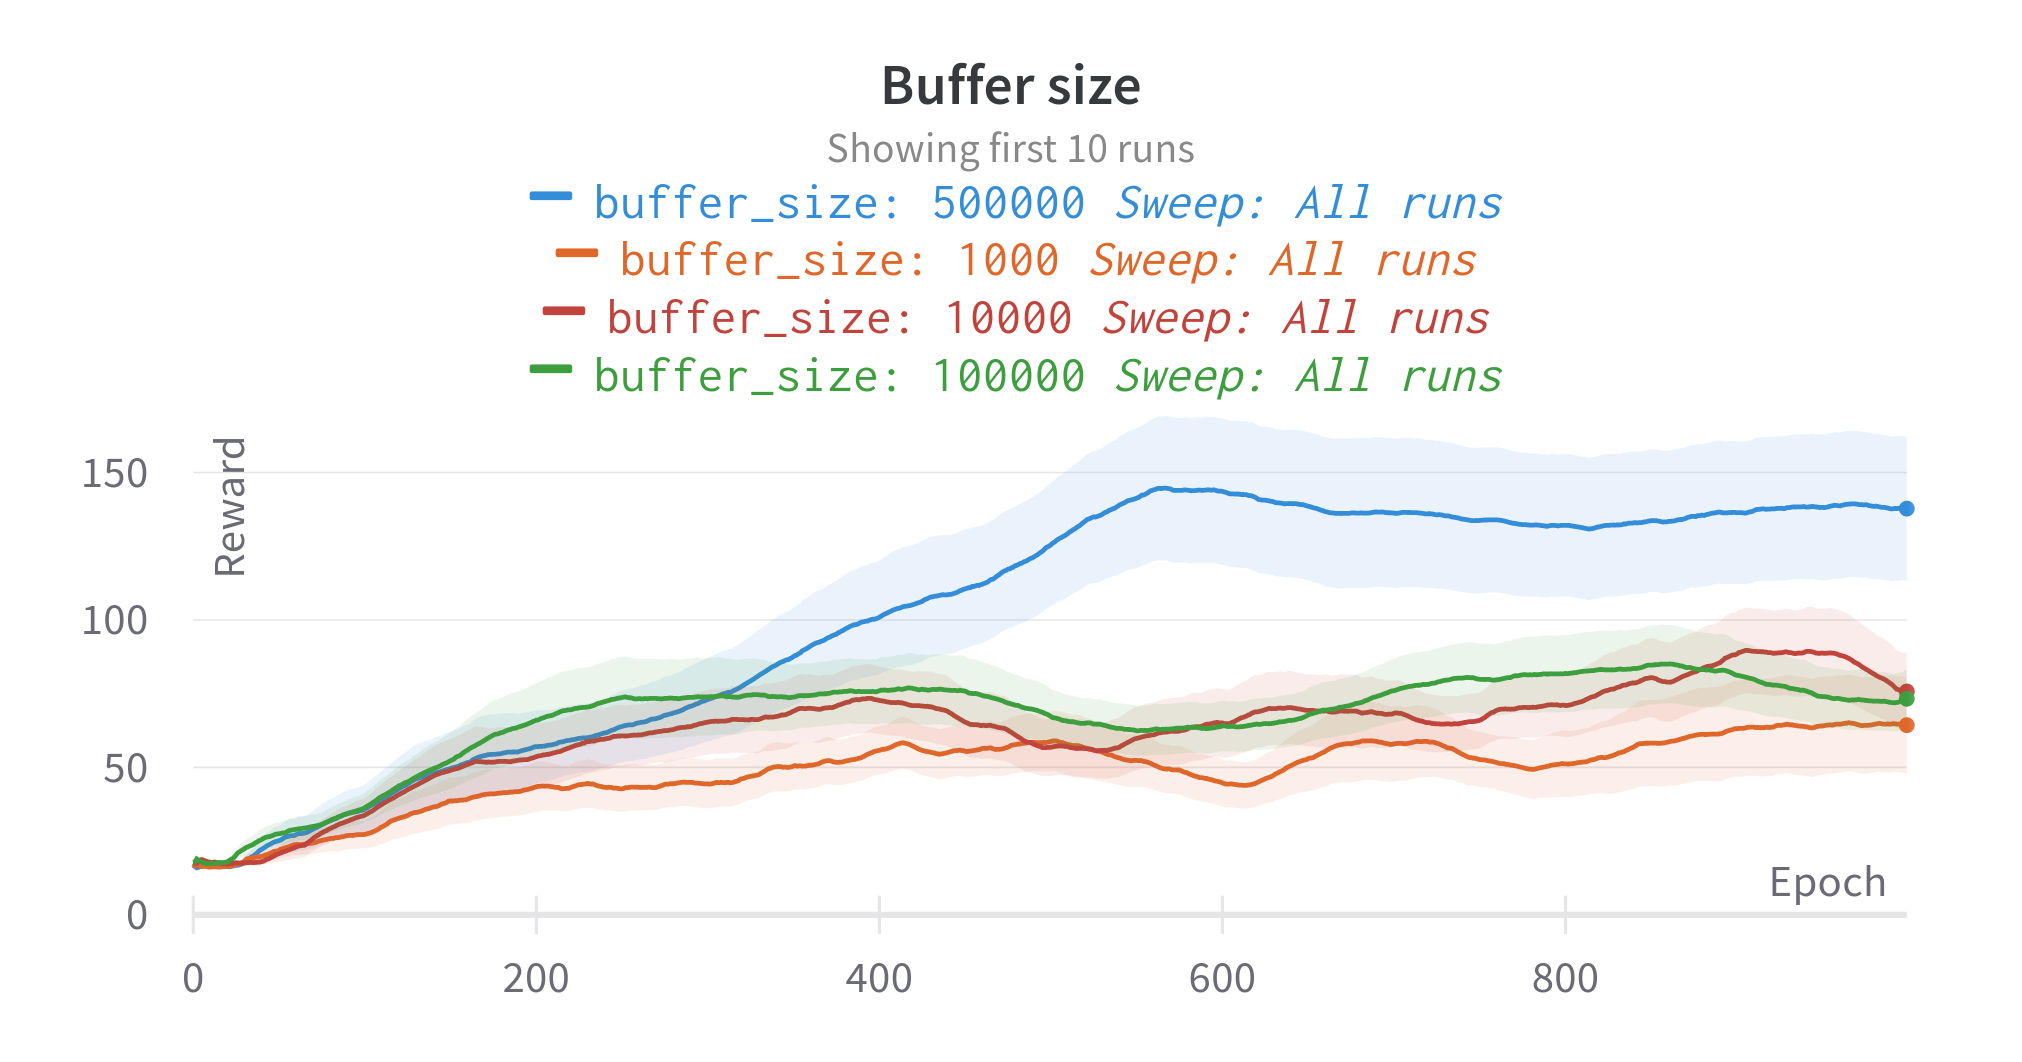
\includegraphics[width=\columnwidth]{assets/hyperparamter-scan/W&B Chart Buffer size.png}
   \caption{The influence of the experience buffer size on the average reward of the last 100 epochs is shown. The values are based on the runs from the hyperparameter scan.
   }
   \label{fig:hyperparameter_scan_isolated_buffer_size}
\end{figure}

\begin{figure}[ht!]
   \centering
   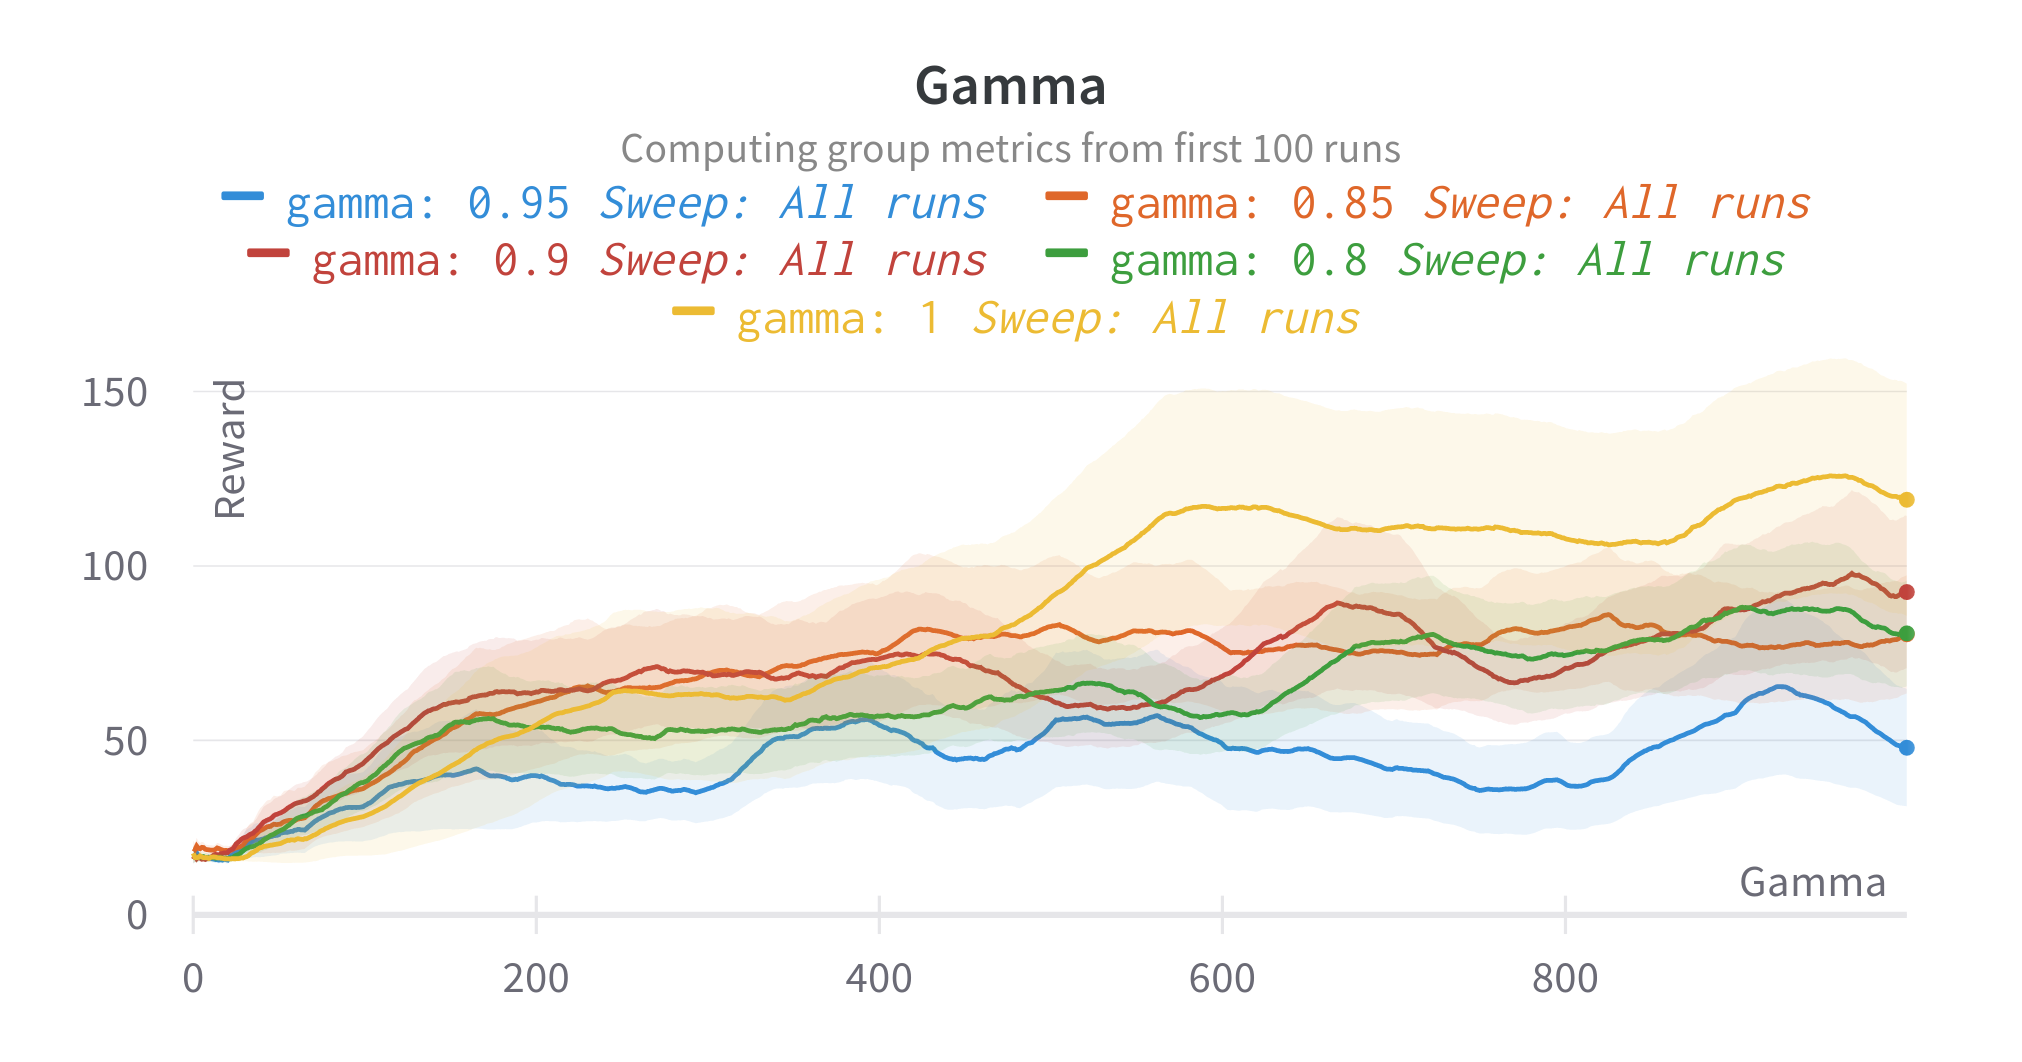
\includegraphics[width=\columnwidth]{assets/hyperparamter-scan/W&B Chart Gamma.png}
   \caption{The influence of gamma on the average reward of the last 100 epochs is shown. The values are based on the runs from the hyperparameter scan.
   }
   \label{fig:hyperparameter_scan_isolated_gamma}
\end{figure}

\section{Discussion}
\label{sec:discussion}
% Discuss results in summary here


% Improvements
%   Use soft update from PolicyNet to Target net instead of hard copy every x epochs
%   Use early stopping to limit effect of overfitting and catastrophic forgetting and reduce computation time
%   Use other Optimizer (SGD) and loss metric (Huber-loss)
%   Decrease size of hyperparameter scan search space or run significantly more runs


% In the unusual situation where you want a paper to appear in the
% references without citing it in the main text, use \nocite
\nocite{DBLP:books/sp/Plaat22}

\bibliography{main}
\bibliographystyle{icml2021}


\appendix
\section{Hyperparameter Scan Results}
\label{sec:hyperparameter-scan-results}

% TODO Move into main part if there is enough space
\begin{figure*}[ht!]
   \centering
   \includegraphics[width=\textwidth]{assets/hyperparamter-scan/W&B Chart parallel axis.png}
   \caption{Parallel axis plot of the hyperparameter scan. 
      Each line shows a single parameter configuration that was evaluated. 
      The color indicates the performance measured by the average of the last 100 epochs (see legend on the right). 
      Higher average reward (yellow) is better.
      Configurations with an average reward of more than 150 are highlighted (see selection on the legend).
      There is an interactive version of this graph available online at \url{https://api.wandb.ai/links/rl-leiden/udme67qe}.
   }
   \label{fig_hyperparameter_scan_parallel_axis}
\end{figure*}


\section{Team member contributions}
Tommaso and Andrija implemented the DQN with ER and TN, experiment configs and executed experiments.
Tom implemented plotting, improved the DQN implementation, executed experiments and did the hyperparameter scan with Weights and Biases.
Everybody designed and configured the experiments.
The report was written with equal contribution from everyone.


\end{document}


% This document was modified from the file originally made available by
% Pat Langley and Andrea Danyluk for ICML-2K. This version was created
% by Iain Murray in 2018, and modified by Alexandre Bouchard in
% 2019 and 2021. Previous contributors include Dan Roy, Lise Getoor and Tobias
% Scheffer, which was slightly modified from the 2010 version by
% Thorsten Joachims & Johannes Fuernkranz, slightly modified from the
% 2009 version by Kiri Wagstaff and Sam Roweis's 2008 version, which is
% slightly modified from Prasad Tadepalli's 2007 version which is a
% lightly changed version of the previous year's version by Andrew
% Moore, which was in turn edited from those of Kristian Kersting and
% Codrina Lauth. Alex Smola contributed to the algorithmic style files.
